%!TEX root = ../main.tex

\chapter{Systemarkitektur}

\begin{table}[H]
\centering
{\rowcolors{2}{white!80!black!30}{white!70!black!60} %farver på hver anden række -starter på 3
\setlength{\arrayrulewidth}{0.2mm}					 %tykkelse på linier 
\setlength{\tabcolsep}{10pt}						 %indryk i celle 
\renewcommand{\arraystretch}{1.5}					 %højden på tabelrum
\center
\begin{tabular}{|p{4cm}|p{4cm}|p{4cm}|}		 %længden på alle rum
\hline

\multicolumn{3}{|>{\columncolor{white!20!black!90}}m{13.44cm}|}{\textcolor{white}{\large{\textbf{Revision}}}} \\\hline
\rowcolor{white!70!black!60}
\textcolor{black}{\large{\textbf{Ændret af}}}&
\textcolor{black}{\large{\textbf{Version}}}&	
\textcolor{black}{\large{\textbf{Dato}}}\\
\hline
Alle	& 0.1	 	& 17-03-2015  \\
		& 		&   \\
		& 		&   \\
		& 	 	&   \\
\hline
\end{tabular}
}
\caption{Revision for Systemarkitektur}
\label{table:RevSys}
\end{table}

\section{System diagrammer}

%!TEX root = ../../main.tex

\subsection{System Domænemodel}

\systemDomainModel{0.82}{System}{AVS}

\subsection{System BDD}

\systemBDD{0.82}{System}{AVS}

\subsubsection{CentralControl}
CentralControl er systemets centrale computer. Det er gennem dette delsystem, at brugerens interaktion bliver behandlet og formidlet videre til andre delsystemer. CentralControl driver en webserver med dertilhørende web-applikation (GUI), som tillader brugeren at interagere med systemet gennem sin web-browser. Webserveren kommunikerer med et stykke centralt software, FlexPMS.

\subsubsection{GUI}
GUI er den brugergrænseflade, som brugeren kan tilgå systemet gennem.

\subsubsection{FlexPMS}
FlexPMS (Flexible Plant Management System) softwaren er bindeleddet mellem GUI og de andre delsystemer. FlexPMS afvikles konstant på CentralControl, og håndterer at sende kommandoer til og opsamle data fra KarControl. FlexPMS kommunikerer med de andre delsystemer gennem enhedsdrivers, som er udviklet til – og installeret på – CentralControl.

\subsubsection{Database}
Databasen gemmer alle indstiller lavet af brugeren gennem GUI.

\subsubsection{KarControl}
KarControl er en styring, som formidler og håndterer al datakommunikation og kommandoer relateret til ét kar. KarControl formidler kommandoer sendt fra CentralControl videre til hardware koblet på det pågældende kar (f.eks. at åbne og lukke for ventiler), samt formidler måledata fra sensorer tilbage til CentralControl. KarControl ved hvilken pH-værdi karret skal have, samt hvilken koncentration af gødning og jordfugtighed planterne, der er tilkoblet karret, skal have. KarControl sørger selv for, at vedligeholde disse værdier. CentralControl giver KarControl besked, når der foretages ændringer af disse værdier.

\subsubsection{Sensor Ø}
Sensor Ø’er giver mulighed for at måle (f.eks. jordfugtighed) over et større areal ved, at Sensor Ø’erne spredes over området, hvor planterne gror, og har hver især tilsluttet sensorer. Dermed kan man måle jordfugtighed lokalt for området omkring Sensor Ø’en og styre vandtilførslen specifikt for planterne, som står i området.

\subsubsection{RSConverter}
RSConverter konverterer fra RS485 til RS232 når der modtages data, og fra RS232 til RS485 når der afsendes data.


\subsection{System Allokeringsdiagram}

\systemAllokeringsDiagram{0.82}{System}{AVS}









\newpage

\section{Kar Control diagrammer}

%!TEX root = ../../main.tex

\subsection{KarControl BDD}
\systemBDD{0.82}{KarControl}

\subsubsection{KarGruppe}
KarGruppe er den overordnede betegnelse for et vandkar med tilførende pH-værdi og gødningskoncentration. KarGruppen består af diverse sensorer og aktuatorer, og styrer et vilkårligt antal Sensor Ø’er. KarGruppen er styret af en controller, KarControl.

\subsubsection{Indløbsventil}
Indløbsventilen åbner og lukker for vandtilføjelsen til karret. Den bruges i forbindelse med, at der skal fyldes vand på karret. Det antages, at indløbsventilen er tilsluttet en vandforsyning, som altid er åben.

\subsubsection{Afløbsventil}
Afløbsventilen åbner og lukker for, at vand kan løbe ud af karret. Den bruges i forbindelse med, at karret skal tømmes.

\subsubsection{pH-Sensor}
pH-sensoren målet pH-værdien af gødningsblandingen i karret.

\subsubsection{Vandpumpe}
Vandpumpen pumper vand fra karret ud til Sensor Ø’erne.

\subsubsection{Flowmåler}
Flowmåleren måler mængden af vand, som tilføres karret gennem Indløbsventilen.

\subsection{KarControl IBD}
\systemIBD{0.82}{KarControl}{KarControl}

\subsubsection{RSIn}
RSConverter konverterer mellem RS485 og UART 232 når der skal kommunikeres med CentralControl.

\subsubsection{RSOut}
RSConverter konverterer mellem RS485 og UART 232 når der skal kommunikeres med Sensor Ø'er.

%\subsection{KarControl Allokeringsdiagram}
%\systemAllokeringsDiagram{0.82}{KarControl}{KarControl}

\subsection{Signalbeskrivelser KarControl}
\systemSignaler{KarControl} {
KarBus				& RS485 bus til kommunikation mellem enheder & Binary 1 (OFF)
																   (Voa-Vob<-200 mV)
																   Binary 0 (ON)
																  (Voa-Vob>+200 mV)	 	& Differentielt bussystem \\
OeBus				& RS485 bus til kommunikation mellem enheder & Binary 1 (OFF)
																   (Voa-Vob<-200 mV)
																   Binary 0 (ON)
																  (Voa-Vob>+200 mV)	 	& Differentielt bussystem \\
Data485				& RS485 bus til kommunikation mellem enheder & Intern:SW-signal		& Internt signal fra RSconverter til KarGruppe \\
Data232				& RS485 konverteret til logisk niveau		 & Intern:SW-signal 	& Konverteret signal fra RSconverter til Controller  \\
EnableIndløb		& Signal til at lukke vand ind i kar		 & Logisk:0-5V			& Signal til styring af Indløbsventil   \\
EnableAfløb			& Signal til at lukke vand ud af kar		 & Logisk:0-5V			& Signal til styring af Afløbsventil   \\
EnableVandpumpe		& Styre signal til pumpe			   	     & Logisk:PWM 0-5V 		& Signal til PWM-styring af Vandpumpe	\\
Puls				& Takttæller af flow				   	 	 & Logisk:0-5V 			& Retursignal fra flowtæller \\
pH					& Analog signal fra pH måler			 	 & Analog:-420mV-420mV  & Analogt sensorsignal \\
Indløb				& vandstyring i kar							 & Vandflow   			& Vandtilførsel til karret \\
Afløb				& vandstyring i kar	 						 & Vandflow  			& Vandtilafledning fra karret \\
Dossering			& vandstyring til planter					 & Vandflow    			& Vandtilførsel til dosering \\
}

\newpage

\section{SensorØ diagrammer}

%!TEX root = ../../main.tex

\newpage

\section{pH-sensor diagrammer}

%!TEX root = ../../main.tex

\newpage

\section{jordfugtigheds-sensor diagrammer}

%!TEX root = ../../main.tex

\newpage

\section{Ventil diagrammer}

%!TEX root = ../../main.tex

\subsection{Ventilstyring BDD}

\begin{figure}[H]
	\centering
	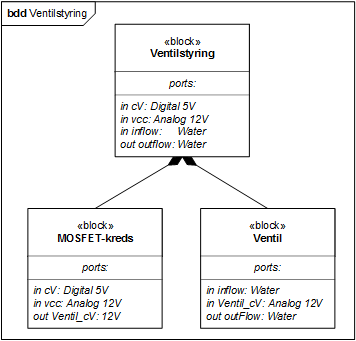
\includegraphics[width=0.82\textwidth]{Systemarkitektur/Ventiler/Ventilstyring_BDD.png}
	\label{fig:Ventilstyring BDD}
	\caption{Block Definition Diagram af Ventilstyring}
\end{figure}



\subsection{System IBD}

\begin{figure}[H]
	\centering
	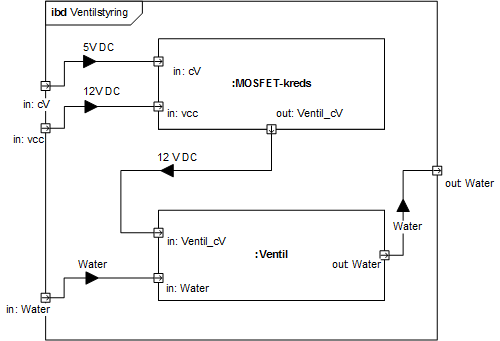
\includegraphics[width=0.82\textwidth]{Systemarkitektur/Ventiler/Ventilstyring_IBD.png}
	\label{fig:Ventilstyring IBD}
	\caption{Internal Block Diagram af Ventilstyring}
\end{figure}



\subsection{System Flowchart}

\begin{figure}[H]
	\centering
	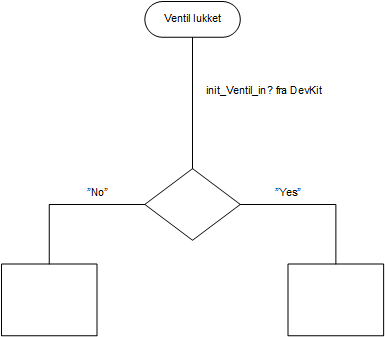
\includegraphics[width=0.82\textwidth]{Systemarkitektur/Ventiler/Ventilstyring_Flowchart.png}
	\label{fig:Ventilstyring FC}
	\caption{Flowchart af Ventilstyring}
\end{figure}

\newpage

\section{Vandpumpe diagrammer}

%!TEX root = ../../main.tex

Vi bruger en vandpumpe på alle vores kar.

\subsection{Vandpumpestyring BDD}

Her under ses et diagram over den generalle opbygning af vandpumpe styringen denne gør sig gældende for alle vandpumper i systemet

\begin{figure}[H]
	\centering
	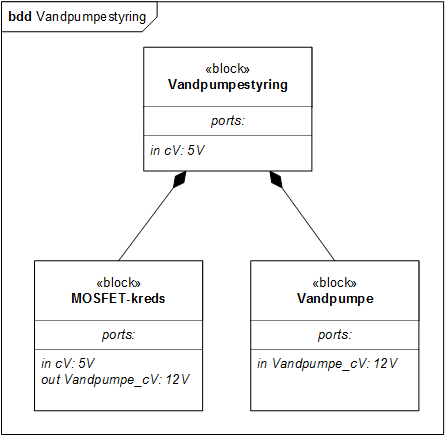
\includegraphics[width=0.5\textwidth]{Systemarkitektur/Vandpumpe/Vandpumpe_BDD.png}
	\label{fig:Ventilstyring BDD}
	\caption{Block Definition Diagram af Vandpumpestyring}
\end{figure}

Her ses så de interne forbindelser i Vandpumpestyringen 

\subsection{Vandpumpestyring IBD}

Her ses så de interne forbindelser i Vandpumpestyringen 

\begin{figure}[H]
	\centering
	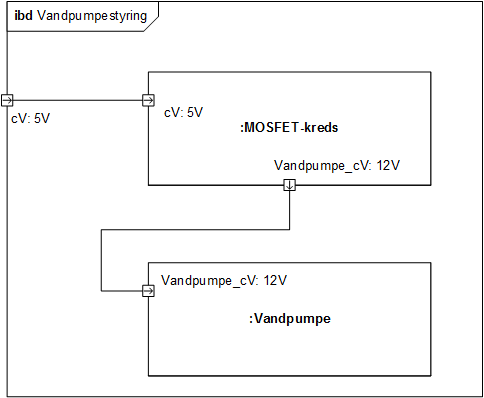
\includegraphics[width=0.5\textwidth]{Systemarkitektur/Vandpumpe/Vandpumpe_IBD.png}
	\label{fig:Vandpumpestyring IBD}
	\caption{Internal Block Diagram af Vandpumpestyring}
\end{figure}




\newpage
%\section{RS485 Converter diagrammer}

\newpage

\section{Teknologi undersøgelser}

%%!TEX root = ../../main.tex
%!TEX root = ../../../main.tex
\subsection{RS485}
Kommunikationen som foregår i systemet imellem brugerinterfacet (Devkit 8000), KarControl (PSoC 4) og de enkelte forgreninger (PSoC 4) skal kunne kommunikere over længere afstande. De allerede kendte busser, SPI og I2C, har begge en maksimal rækkevidde på 1,5m. Vi har derfor været nødsaget til at finde et bedre alternativ. Problemet over længere afstande kan være:

\begin{itemize}
\item Kapacitet i ledningerne
\item Støj fra omkringliggende elektronik
\end{itemize}

For at løse disse problemer, har vi undersøgt RS485-kommunikation. RS485 er en standard som definerer de elektriske karakteristika af sendere og modtagere på en differentiel bus. Ved 2 ledninger kan man opnå half-duplex, og ved 4 ledninger kan man opnå full duplex. Ledningerne i bussen skal være parsnoede. Ved afstande helt op til 1200m, er det muligt at køre med hastigheder på op til 100kbit/s. RS485 er en udbygning af RS422, hvor man har muligheden for at vælge hvorvidt det er input- eller output-driverne som er aktive. Den fysiske konfiguration af bussen skal forbindes som én linje.
Dvs. at man kan f.eks. ikke parallel-forbinde 5 enheder direkte til en master, de skal derimod serieforbindes. Bussen termineres i begge ender, med en modstand som svarer til kablernes egen modstand, normalt 120ohm for parsnoede kabler, imellem de 2 bus-forbindelser.
\\\\
Man vil gerne opnå at masteren er centreret i bussen, og at termineringsmodstandene derved er på 2 slaver. Ved at gøre dette, vil afstanden fra masteren til slaverne være så lille som mulig, og derved vil signal-styrken være bedst.
\\\\
RS485 er KUN en elektrisk definition af bussen, og ikke en kommunikationsprotokol. Dette giver mulighed for at skrive sin egen protokol. Standarden anbefaler dog, at man bruger kommunikationsprotokollen TSB-89.


\fixme{der skal indsættes resten af teknologi undersøgelserne}

